\documentclass[11pt,dvipsnames]{article} % {{{

\usepackage{geometry}
\geometry{total={170mm,240mm}, left=20mm, top=20mm}

\usepackage[utf8]{inputenc}

\usepackage{physics} 
\usepackage{siunitx} 
\usepackage{enumerate} 
\usepackage{pgfplots}
\usepackage{graphicx}
\usepackage{pgfplotstable}
\usepackage{tikz,pgfplots}
\usepackage{amsmath} 
\usepackage{xcolor}
\usepackage{float}
\usepackage{amsfonts}
\usepackage{dsfont}
%\usepackage{bbold}


\newcommand{\fref}[1]{fig.~\ref{#1}}  \newcommand{\tref}[1]{table~\ref{#1}}
\newcommand{\Fref}[1]{Fig.~\ref{#1}}  \newcommand{\Tref}[1]{Table~\ref{#1}}

\newcommand{\h}[1]{\colorbox{Yellow}{#1}}
\newcommand{\1}{\mathds{1}}

\usepackage[]{lineno}  \linenumbers
\setlength\linenumbersep{3pt}
	

\usepackage{fancybox}
\usepackage{colortbl}
\usepackage{amsbsy}
\usepackage[draft,inline,nomargin]{fixme} \fxsetup{theme=color}
\FXRegisterAuthor{cp}{acp}{\color{blue}CP}
\FXRegisterAuthor{ja}{aja}{\color{RedViolet}JA}
% }}}
\begin{document}
% Titulo y otros {{{
\title{Projective maps on a system of $n$ qubits} 
%Title should be concise and to the point  
\author{J. A. de León\\ \small{in collaboration with C. Pineda, D. Dávalos, A. Fonseca}}


\date{\today}  

\maketitle
% }}}
% Intro {{{
According to \cite{bengtsson_zyczkowski_2017}, an arbitrary density matrix on $n$  
qubits can be expanded as
\begin{align}
  \rho = \frac{1}{2^n}\1 + \sum _{i=1}^{2^{2n}-1}\tau _i\sigma _i,
	\label{rho}
\end{align}
where we'll identify $\sigma _i$ as the tensor products of Pauli 
matrices, which form a basis of the space of traceless Hermitian
%\cpnote{Quitar density}
%density 
matrices, and 
$\tau_i$ the projections of $\rho$ onto each element of this basis.

%where the sum is over vectors $\vec{v}=\qty(v_1,\cdots, v_n)$ with entries
%$v_i$ chosen from the set $\{0,1,2,3\}$. We label the coefficients $\Tr \qty(
%\sigma _{v_1} \otimes \sigma_{v_2} \otimes \cdots \otimes \sigma_{v_n}
%\rho )$ as $r_{v_1, v_2,\ldots, v_n}$ to shorten the notation. 


In this work, we are interested in studying the set of maps that erase
some components $\tau_i$ in $\rho$ and characterize the subset of maps
that are quantum channels. We'll refer to the coefficients in both terms of 
\eqref{rho} as the components in $\rho$. 
For 1 qubit the picture of our problem is easy to understand given that 
$\tau_i$ are the components of a vector in the Bloch ball, the so-called
Bloch vector. As an example, let's consider a map that erases any of the 
components of the Bloch vector. Geometrically, this map collapses 
the Bloch ball into a disk. This operation does not fulfill 
the condition of complete positivity and therefore is not a quantum channel.  

%The kind of maps that act on density matrices of the form \eqref{rho} that
%we're interested in are those which leave invariant or erase  
%components
%in $\rho$ (i.e. $r'_{v_1, v_2,\ldots, v_n}=r_{v_1, v_2,\ldots, v_n}$ or
%$r'_{v_1, v_2,\ldots, v_n}=0$, where the primed $r$'s refer to the 
%components in the transformed density matrix $\rho '$). 

So far, with a numerical method we've characterized all 1 and 2 qubit maps, 
whereas for 3 qubits system we have numerically analyzed only maps that leave 
invariant 1, 2, 3, 4, and 64 components in $\rho$. Nonetheless, we have strong
indications that point that only the maps that leave invariant 8 components are 
needed to analyze in order to find the complete set of 3-qubit quantum 
channels.
% }}}
\section*{Results} % {{{
In \fref{fig:pictorial-rep-rho} we introduce a pictorial representation 
of the identity map acting on a density matrix of a system of 1, 2 and 3 qubits,
respectively. It will be helpful to visualize the maps we are studying 
making use of this tool. We'll consider any little square or cube in blank
as a component erased in $\rho$ by the map. 
In the following subsections we present the actual quantum channels of
1 and 2 qubits, and preliminary results for 3 qubits.
\begin{figure}[H] % {{{
	\centering
	\hfill \hfill
	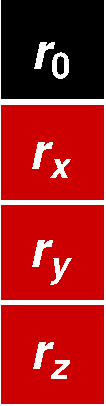
\includegraphics[height=2.5cm]
	{img/tablero-1q}
	\hfill
	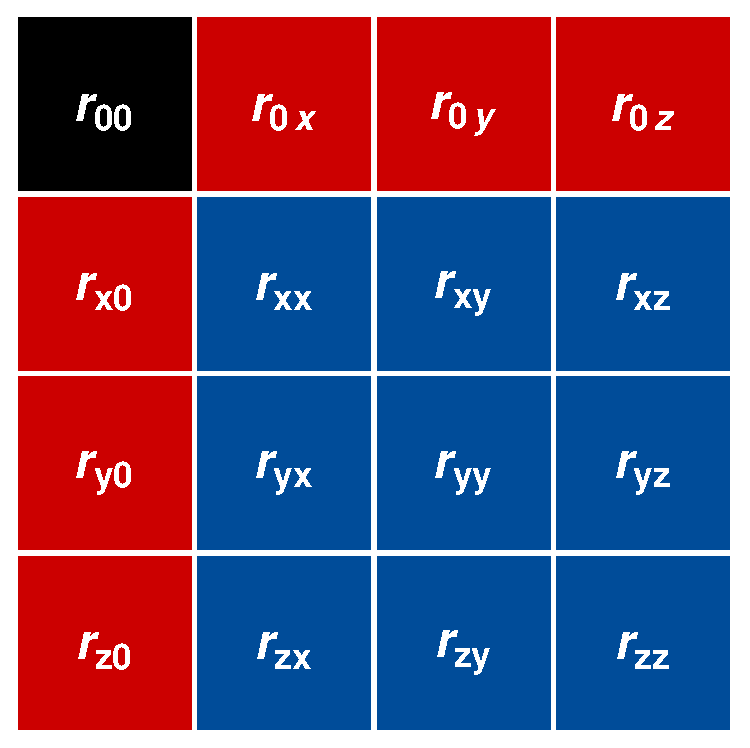
\includegraphics[width=2.5cm]
	{img/rho2q(2)}
	\hfill 
	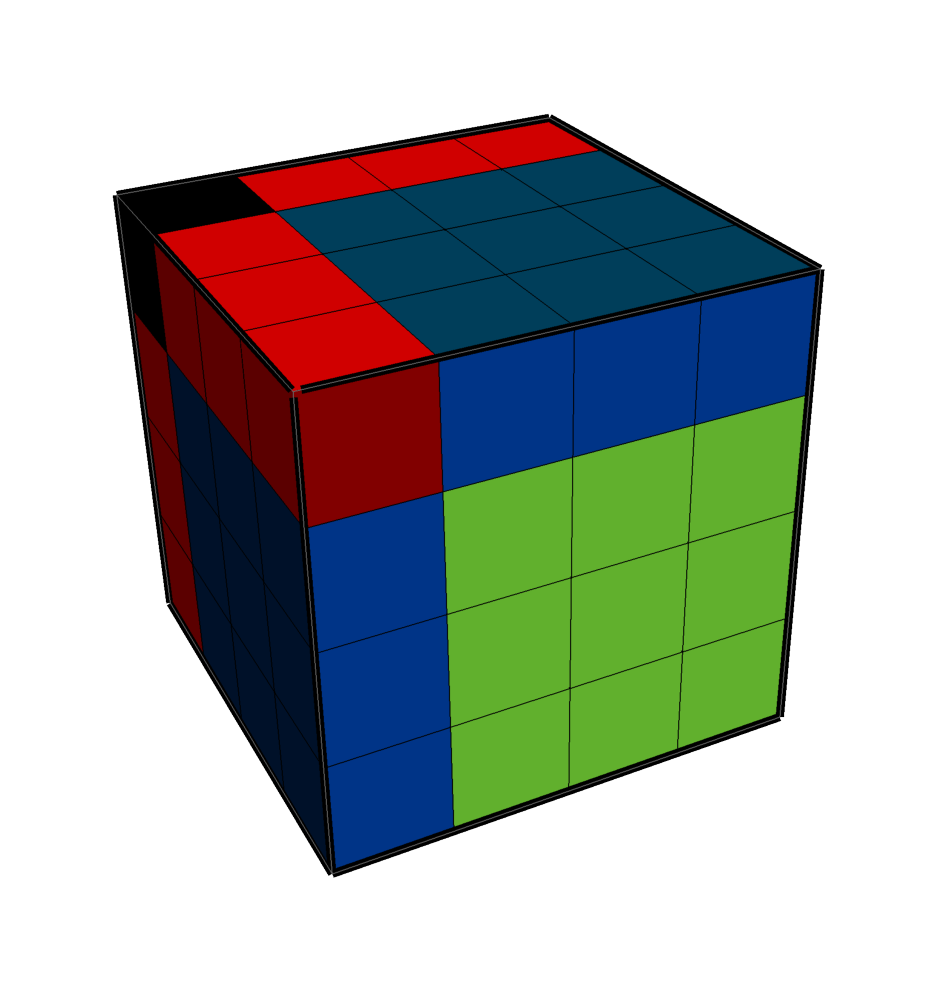
\includegraphics[width=2.5cm]
	{img/rho-3q}
	\hfill \hfill
	\caption{From left to right the identity map acting on
  an arbitrary density matrix of 1, 2 and 3 qubits, respectively. 
	Red squares refer to components of local Bloch vectors,
	blue squares to correlations between any pair of qubits and
	green squares to correlations between all qubits in the system, for
	the 3-qubits case. }
	\label{fig:pictorial-rep-rho}
\end{figure} % }}}
\subsection*{1 qubit} % {{{
\begin{figure}[H]% {{{
	\centering
	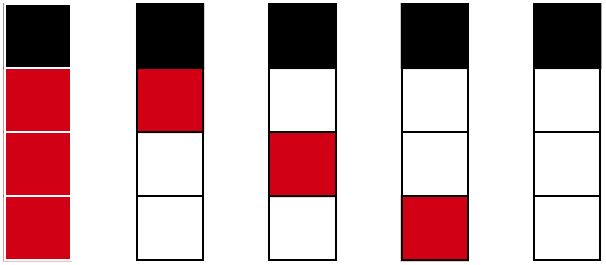
\includegraphics[width=5cm]
	{img/1q-CCs.png}
	\caption{\cpnote{Mejora el caption. } 1-qubit 
quantum channels.
\janote{Listo.}
}
	\label{fig:1q-ccs}
\end{figure} % }}}
The first and last patterns in \fref{fig:1q-ccs} represent the identity 
and completely depolarizing channels. 
In between them, from left to right, the patterns represent 
the bit-phase flip, phase-flip and bit-flip channels, 
all of them for the case $p=0.5$.	
This last three channels are equivalent via permutation
of the components $\tau_i$ of the Bloch vector in \eqref{rho}.
% }}}
\subsection*{2 qubits} % {{{
2-qubits quantum channels have been classified in equivalence classes 
(as shown from \fref{fig:2q-c1} to \fref{fig:2q-c16}) such
that elements in a class are connected by
\begin{enumerate}
	\item Transpositions (particle swaps)
	\item Permutations of rows or columns 1-3 (permutation of individual 
	components) \cpnote{Explica el por que de eso. En los dos casos, mas bien 
di como clasificamos, desde un punto de vista fisico, y luego a que traduice graficamente
eso. primero lo importante y luego el detalle. }
\end{enumerate}
\cpnote{No recuerdo que tan pronto mencionas lo de los colores azules y eso, pero seria 
bueno explicarlo pronto y ser consistente con eso desde la primera figura}

\begin{figure}[H] % {{{
	\centering
  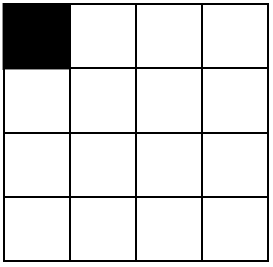
\includegraphics[height=1.2cm]
	{img/C16.png}
	\caption{C${}^{1}$}
	\label{fig:2q-c1}
\end{figure} % }}}

\begin{figure}[H] % {{{
	\begin{minipage}[c]{0.5\textwidth}
		\centering
	  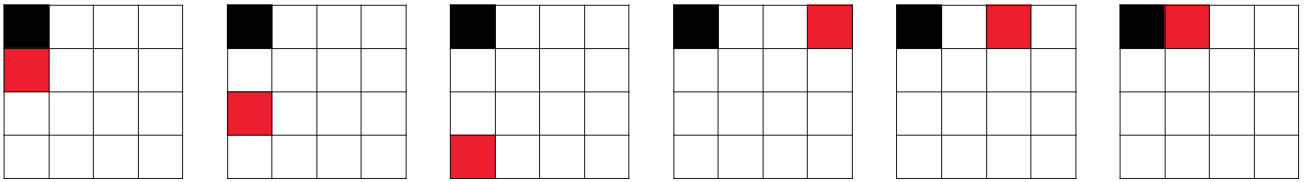
\includegraphics[width=.9\textwidth]
		{img/C12.png}
		\vspace{1.2cm}
		\caption{C${}_1^2$}
	\end{minipage}\hfill
	\begin{minipage}[c]{0.5\textwidth}
		\centering
	  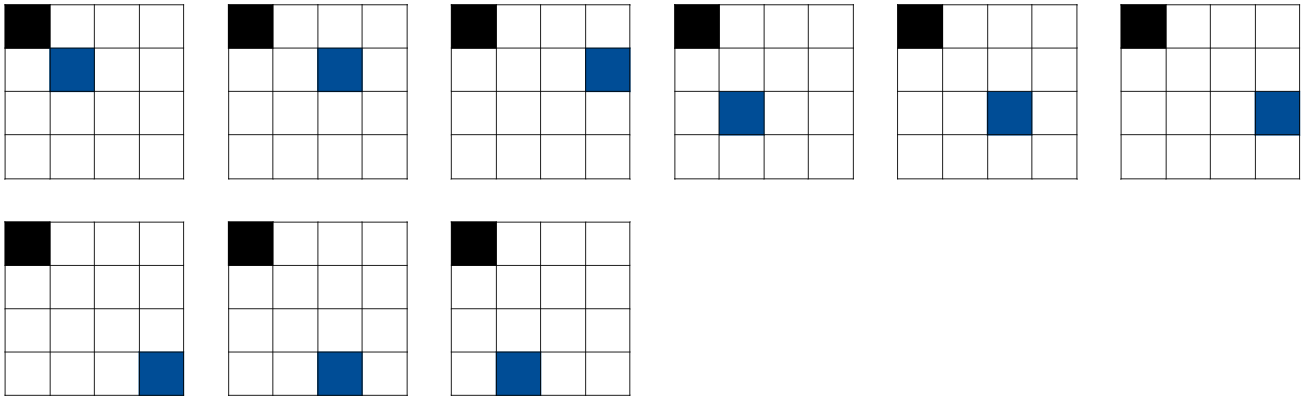
\includegraphics[width=.9\textwidth]
		{img/C22.png}
		\caption{C${}_2^2$}
	\end{minipage}
\end{figure} % }}}

\begin{figure}[H] % {{{
	\begin{minipage}[c]{0.5\textwidth}
		\centering
	  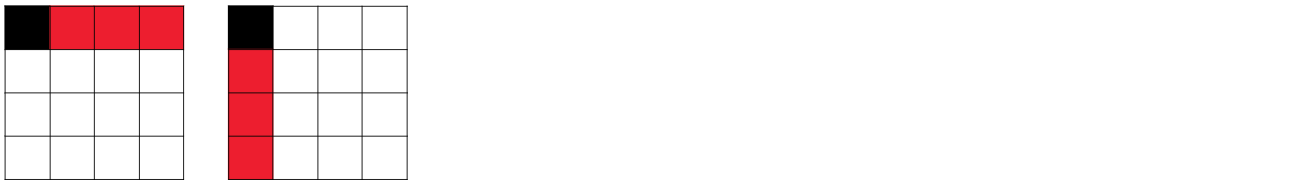
\includegraphics[width=.9\textwidth]
		{img/C14.png}
		\vspace{1.2cm}
		\caption{C${}_1^4$}
	\end{minipage}\hfill
	\begin{minipage}[c]{0.5\textwidth}
		\centering
	  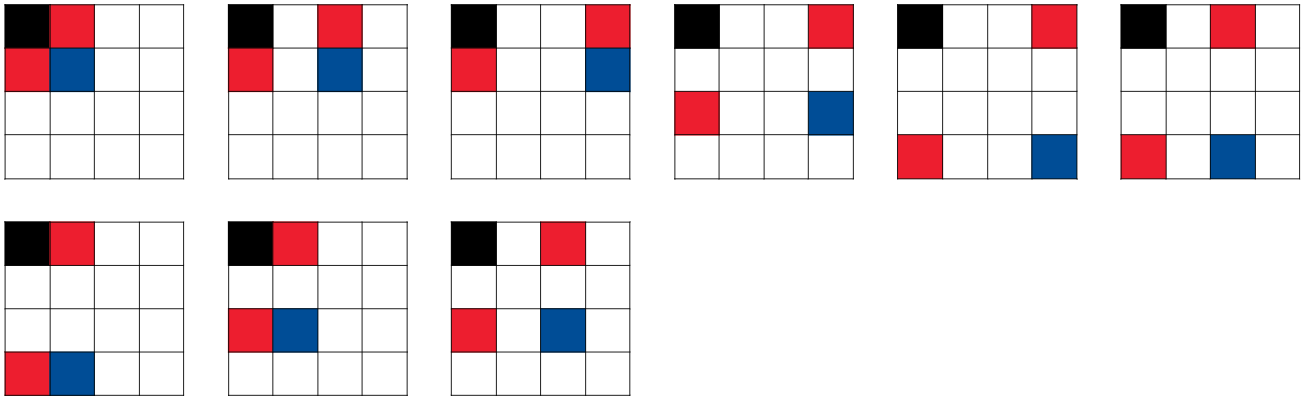
\includegraphics[width=.9\textwidth]
		{img/C24.png}
		\caption{C${}_2^4$}
	\end{minipage}\vfill
\begin{minipage}[c]{0.5\textwidth}
		\centering
	  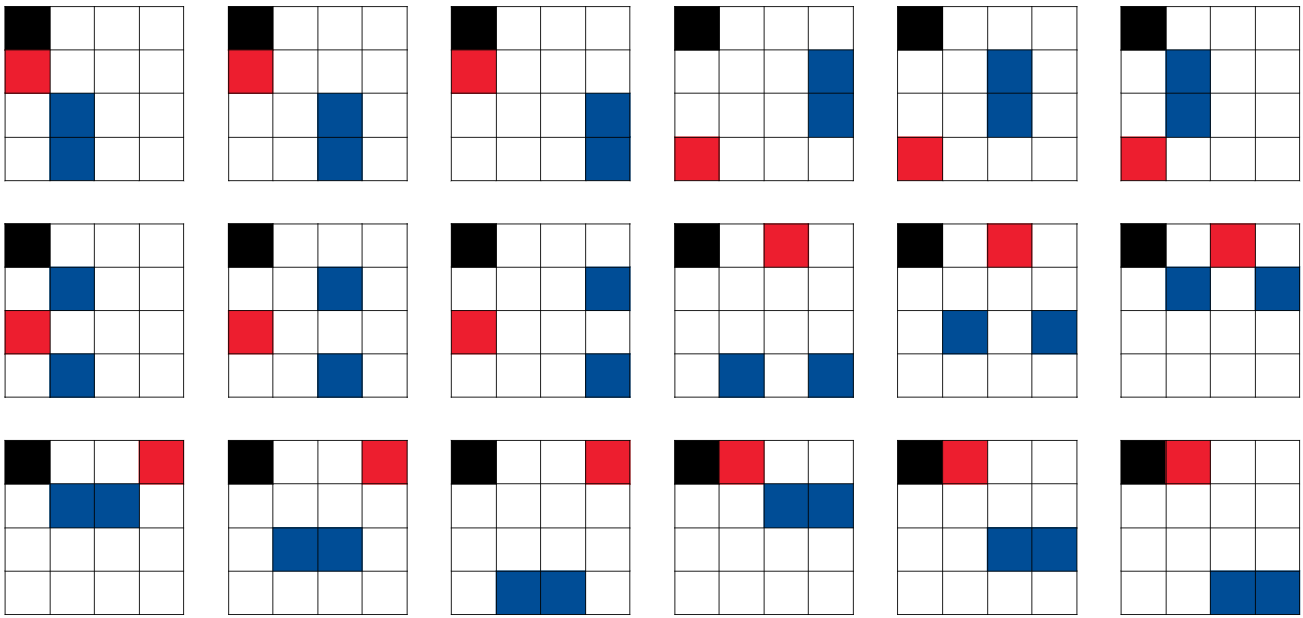
\includegraphics[width=.9\textwidth]
		{img/C34.png}
		\caption{C${}_3^4$}
	\end{minipage}\hfill
	\begin{minipage}[c]{0.5\textwidth}
		\centering
	  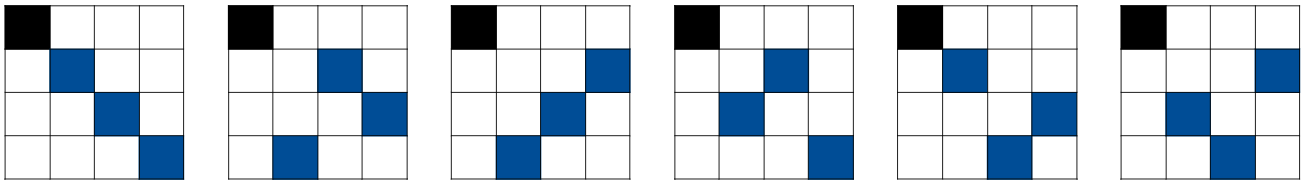
\includegraphics[width=.9\textwidth]
		{img/C44.png}
		\vspace{2.5cm}
		\caption{C${}_4^4$}
	\end{minipage}
\end{figure} % }}}

\begin{figure}[H] % {{{
	\begin{minipage}[c]{0.5\textwidth}
		\centering
	  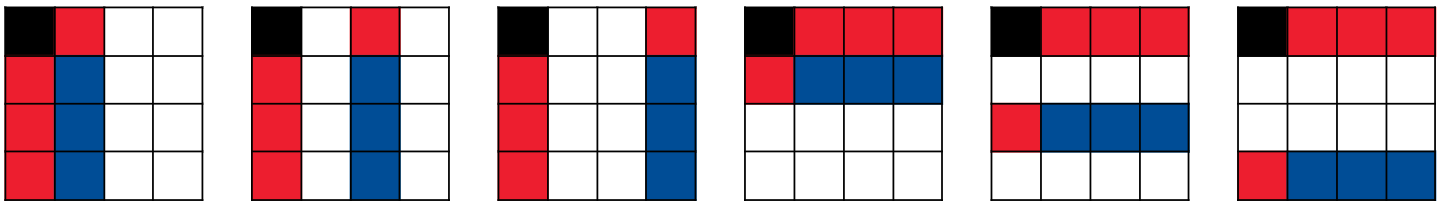
\includegraphics[width=.9\textwidth]
		{img/C18.png}
		\vspace{1.2cm}
		\caption{C${}_1^8$}
	\end{minipage}\hfill
	\begin{minipage}[c]{0.5\textwidth}
		\centering
	  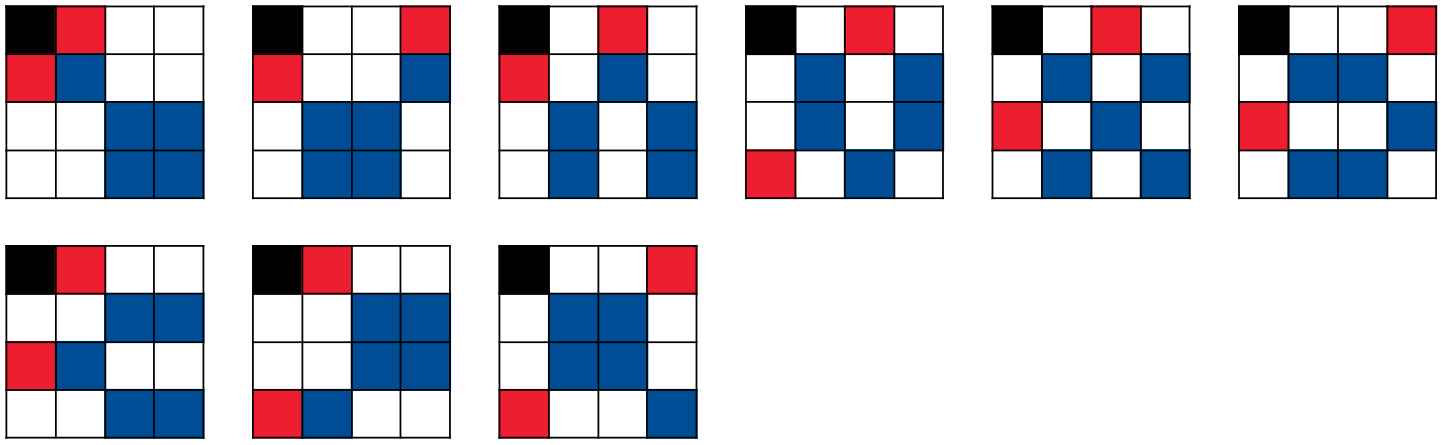
\includegraphics[width=.9\textwidth]
		{img/C28.png}
		\caption{C${}_2^8$}
	\end{minipage}
\end{figure} % }}}

\begin{figure}[H] % {{{
	\centering
  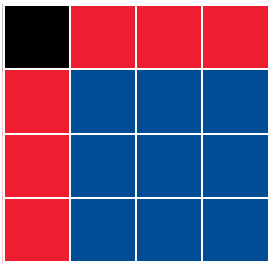
\includegraphics[height=1.2cm]
	{img/C0.png}
	\caption{C${}^{16}$}
	\label{fig:2q-c16}
\end{figure} % }}}

In general, our results exhibit the following features:
\begin{itemize}
\item Only a power-of-2 number of components in $\rho$ 
may be left invariant by quantum
channels. However, not only the number of components in $\rho$ 
to leave invariant determines complete positivity since
not all maps that leave $2^{k}$ components invariant in $\rho$
are quantum channels. For example, the pattern below corresponds 
to a map that is not a quantum channel. \cpnote{Menciona con que clase y que figura
tendría que ocntrastar. También en la siguiente parte sobra el 
ambiente figure, pues ni le pones caption ni quieres que flote. Se lo quité}. % \begin{figure}[H]
% 	\centering
% 	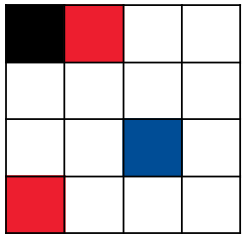
\includegraphics[height=2cm]{img/not-cc}
% \end{figure}
\begin{center}
	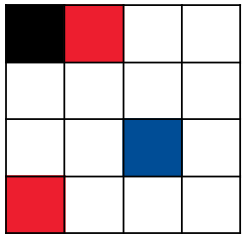
\includegraphics[height=2cm]{img/not-cc}
\end{center}

\item 
The number of valid quantum channels according to the number of components
left invariant are shown in \fref{fig:CCs-by-components}.
\cpnote{ En la figura, creo que los colores sobre y
distraen. Tambien sería padre poner cuantos de cada clase hay. Por ejemplo
poner 1/1 que quiere decir que el unico posible es canal, o 63/128 queriendo
decir que 63 de los 128 son canales.  }

%Two numbers
%of same color correspond to quantum channels that we suspect have a 1:1 
%correspondence. In the next item we extend this discussion.

\begin{figure}[H]% {{{
	\centering
	\begin{tabular}{>{$n=$}l<{\hfill}*{12}{c}}
1 &&&&&\colorbox{Apricot}{1}&3&\colorbox{Apricot}{1}&&&&&5\\
2 &&&&\colorbox{CadetBlue}{1}&\colorbox{Cyan}{15}&35&\colorbox{Cyan}{15}&\colorbox{CadetBlue}{1}&&&&67\\
3 &&&\colorbox{SpringGreen}{1}&\colorbox{RedOrange}{63}&\colorbox{Yellow}{651}&?&\colorbox{Yellow}{¿651?}&
\colorbox{RedOrange}{¿63?}&\colorbox{SpringGreen}{1}&&&?
\end{tabular}
\caption{First column shows the number of qubits in the system.  In the second
column each position correspond to the number of components invariant ($2^0,
2^1, \ldots, 2^{2n}$) and the numbers shown are the number of quantum channels
according to the number of components invariant.  Finally, third column
specifies the total number of quantum channels for a $n$-qubit system.}
\label{fig:CCs-by-components}
\end{figure} % }}}

\item Empirical observations of results for 2 qubits 
led us to some rules that the
patterns showed from \fref{fig:2q-c1} to \fref{fig:2q-c16} obey:
\begin{enumerate}
\item If a component with indices $ij$ is left invariant, then two options are
allowed: \textit{a)} both components with indices $i0$ and $0j$ are left
invariant too, or \textit{b)} both components with indices $i0$ and $0j$ are
erased.
Let's take a look at the next example. \cpnote{Cambié el hfill y los newlines
por un center. Cuando lo veas quita este comentario}
% \newline
% \hfill
\begin{center}
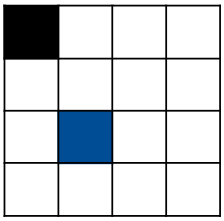
\includegraphics[width=2cm]{img/ex-2q2c-empiricalRule}
\end{center}
% \hfill \hfill
% \newline
The component with indices 21 in the pattern is left invariant,
so the two options allowed are: \textit{a.} components with indices 01 and
20 are erased, as in this pattern above, or \textit{b.} components 
with indices 01 and 20 are left invariant too, 
as in the following pattern 
\begin{center}
% \newline
% \hfill
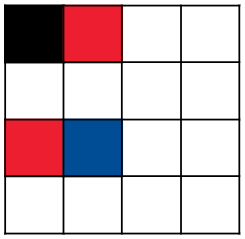
\includegraphics[width=2cm]{img/ex-2q4c-empiricalRule},
% \hfill \hfill 
% \newline
\end{center}
which is another quantum channel.
% \janote{Fin.}

\item Focusing only on the correlation matrix (blue squares): if a component
with indices $ij$ is left invariant and the previous rule is obeyed, then the
remaining components in the correlation matrix on row $i$ and column $j$ must
be erased. 
Let's go back to the last pattern in the previous example. This rule 
ensures that components in the correlation matrix outside of row 2 and 
column 1 may be left invariant by a quantum channel, i.e.
\begin{center}
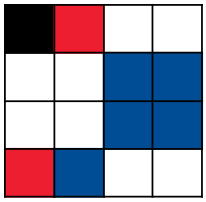
\includegraphics[width=2cm]{img/ex-2q8c-empiricalRule},
\end{center}
which is another quantum channel.
\end{enumerate}	
% Actually, this two simple rules allow us to connect two elements of classes
% C${}^2_k$ and C${}^8_k$. \cpnote{Creo que se pueden hacer más conexiones, no?}
% \janote{Es cierto, corrijo:}
Actually, this two simple rules allow us to relate
different equivalence classes. In the previous example we were able to connect 
an element of C${}_2^2$ to one of C${}_3^4$, to another one of
C${}_2^8$.

% \janote{Agrego el siguiente item porque no le había dado la suficiente
% importancia unos items arriba (en el de la fig. 13)}
\item \textit{(Rainbow hypothesis)} Quantum channels
that leave $2^k$ components invariant and $2^{2n-k}$ have a
1:1 correspondence. That is to say, two numbers of the same color 
in \fref{fig:CCs-by-components} correspond to quantum
channels that have a 1:1 correspondence. 

\item The action of a quantum channel on every subsystem must be another
channel. 
% \cpnote{Esto también hay que explicar que efecto tiene en los diagramas}
% \janote{\h{Inicio}}
This can be seen from the patterns in \fref{fig:2q-c1} to \fref{fig:2q-c16}.
Recall that red squares represent components of local Bloch vectors 
and blue squares represent correlations shared between qubits. 
Then, it may be noted that in the first column and first row of every
pattern there is a 1-qubit quantum channel, of the form of \fref{fig:1q-ccs}.
% \janote{\h{Fin}}
\end{itemize}
% }}}
\subsection*{3 qubits} % {{{

Recall that for 3 qubits system we have numerically analyzed only maps that
leave invariant 1, 2, 3, 4, and 64 components in $\rho$. Therefore, results
presented in this section are preliminary. Quantum channels follow the same
features of 2 qubits system. Not all 3 qubits quantum channels are shown as in
the previous section, but only one element of every equivalence class found.
Elements in equivalence classes are connected via particle swaps and
permutation of individual components.

\subsubsection*{1-invariant-component maps} % {{{
The only map that leaves invariant 1 component in $\rho$ is the completely
depolarizing channel.
\begin{figure}
	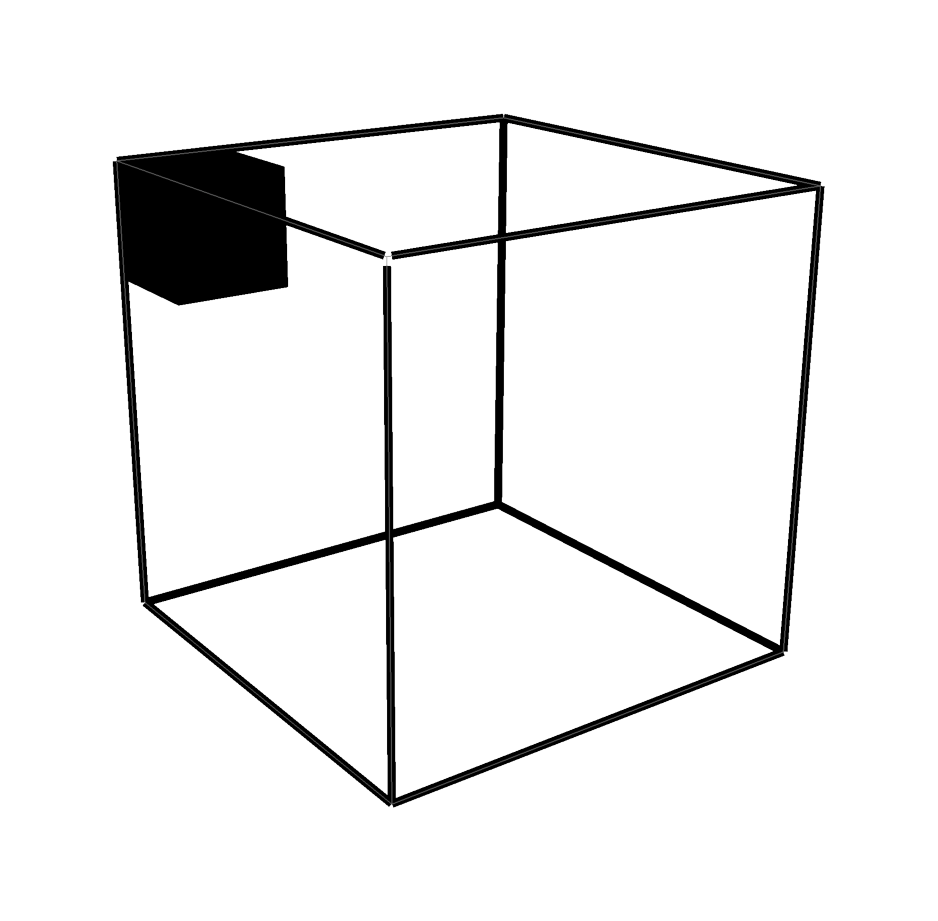
\includegraphics[height=4cm]{img/3q-1c}
	\caption{Completely depolarizing channel for 3 qubits.}
	\label{fig:QC-3q-1c}
\end{figure}
% }}}
\subsubsection*{2-invariant-components maps}% {{{
All 63 maps that leave invariant 2 components in $\rho$ are 
quantum channels. It's important to mention that in the 2 qubits case all 
2-invariant-components maps are quantum channels, too. We can distinguish
3 equivalence classes: quantum channels that leave invariant
\begin{enumerate}
	\item any component of a local Bloch vector,
	\item any correlation between any pair of qubits,
	\item any correlation between all qubits in the system.
\end{enumerate}
\begin{figure}[H]
	\centering
	\hfill \hfill
	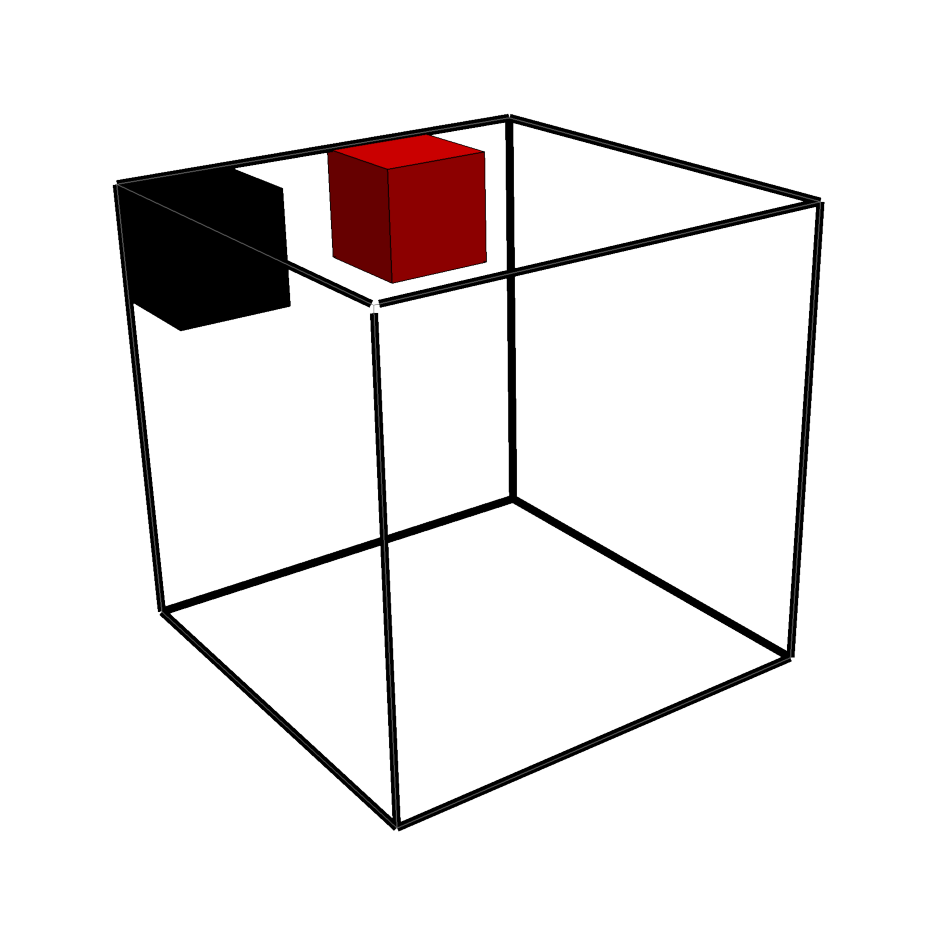
\includegraphics[height=4cm]{img/3q-2c-1}
	\hfill
	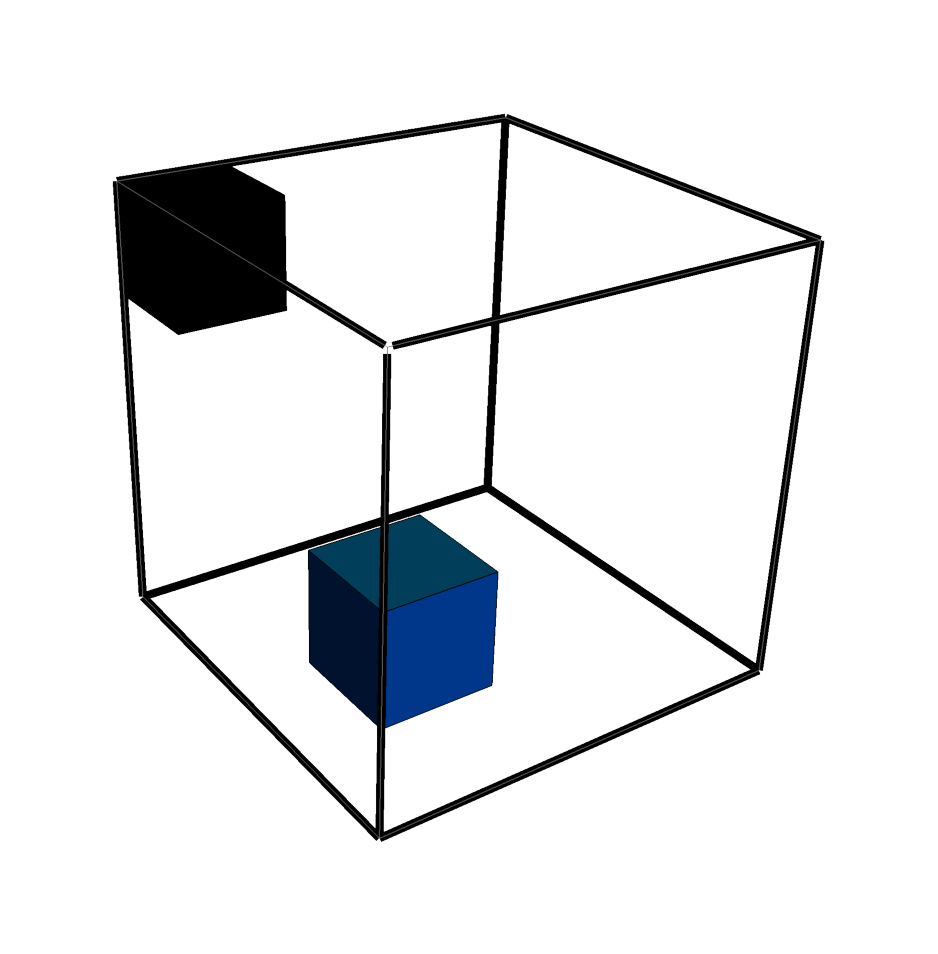
\includegraphics[height=4cm]{img/3q-2c-2}
	\hfill
	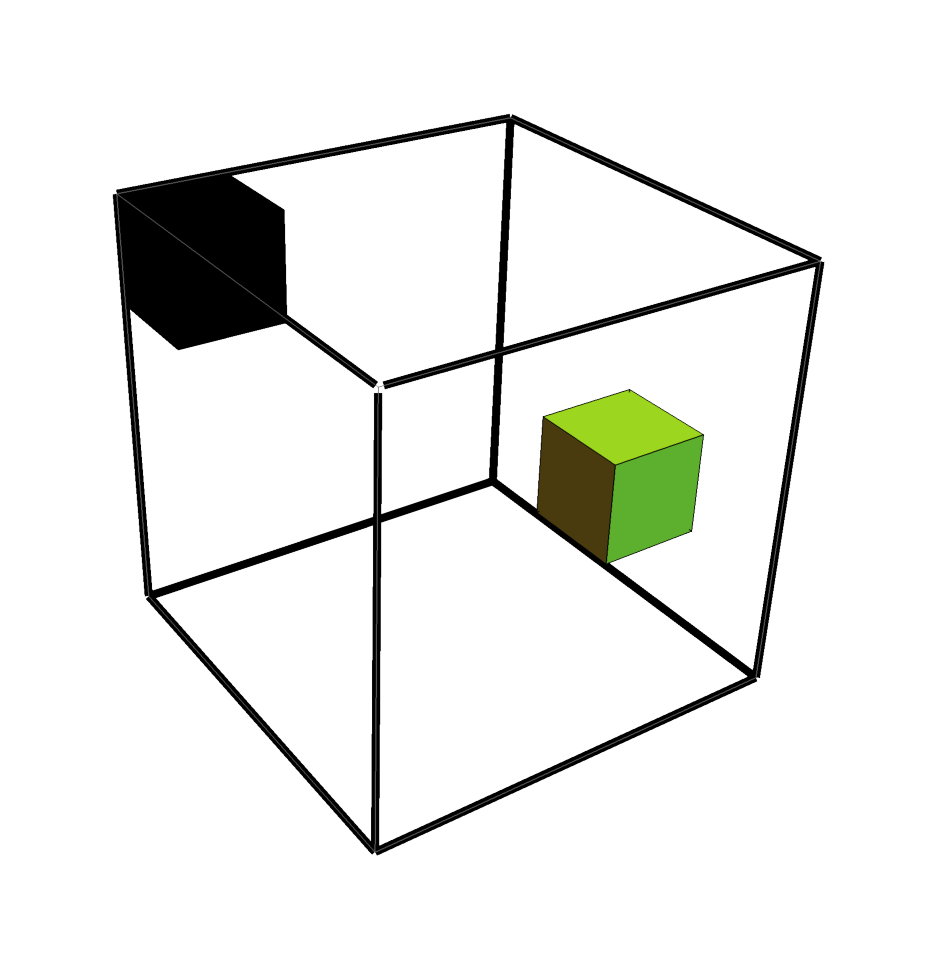
\includegraphics[height=4cm]{img/3q-2c-3}
	\hfill \hfill
	\caption{3-qubits quantum channels. One element of each of the 
	3 equivalence classes 
	(from left to right): leaves invariant one component of any local
	Bloch vector, one correlation between any pair or qubits, and 
	one correlation between all qubits in the system.}
	\label{fig:QC-3q-2c}
\end{figure}

% }}}

\cpnote{Estudiates los que dejan invariantes 3 elementos?}

\subsubsection*{4-invariant-components maps} % {{{
There are 39,711 maps that leave invariant 4 components in $\rho$, 651
are quantum channels and may be classified in 10 equivalence classes.
One arbitrary element of each class is shown in \fref{fig:QC-3q-4c}. 
We understand how to infer 5 out of the 10 classes from quantum channels
of 1 and 2 qubits, as it will be discussed.


On top of the figure the first 4 elements
(from left to right) correspond to quantum channels that are separable
in a 1 or 2 qutbis quantum channel acting on any subsystem 
and a completely depolarzing channel acting on the rest of the system.
The fifth element on top of \fref{fig:QC-3q-4c} may be inferred from
an extension for 3 qubits of one of the empirical rules stated for 2 qubits: 
\begin{itemize}
	\item If a component with indices $ijk$ (all different from zero) is
	left invariant by the channel, if and only if one of the cases must be followed:
	\begin{enumerate}
		\item No other component is left invariant (i.e. a 2-invariant-components
		channel),
		\item Components $0j0$ and $i0k$ are also left invariant,
		\item Components $00k$ and $ij0$ are also left invariant,
		\item Components $i00$ and $0jk$ are also left invariant,
		\item Components $ij0$, $0jk$, $i0k$, $i00$, $0j0$, and
		$00k$ are left invariant.
	\end{enumerate}
	Be noted that case 5 leads to a quantum channel that leaves invariant
	more than 4 components in $\rho$.
\end{itemize}
Quantum channels belonging to equivalence classes of bottom elements in 
\ref{fig:QC-3q-4c} are such that we still can't infer with what has 
been understood for 2 qubits.

\begin{figure}[H]
	\centering
	\hfill \hfill
	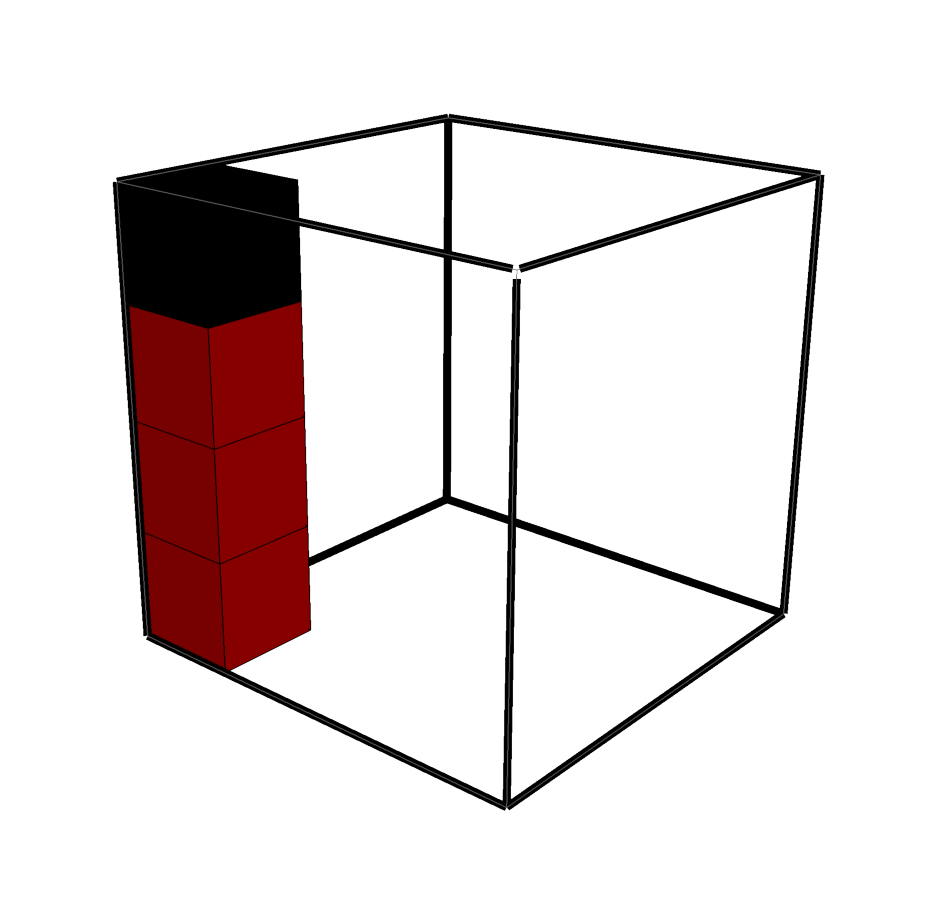
\includegraphics[height=3cm]{img/3q-4c-si-1}
	\hfill
	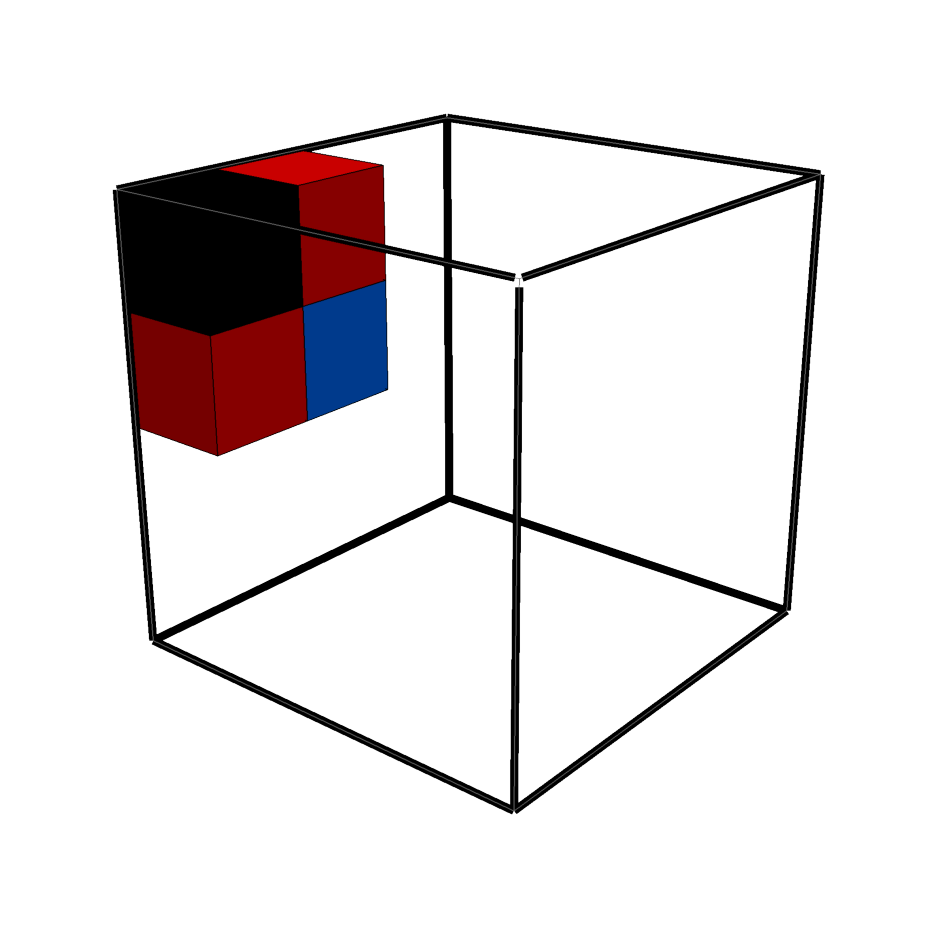
\includegraphics[height=3cm]{img/3q-4c-si-2}
	\hfill
	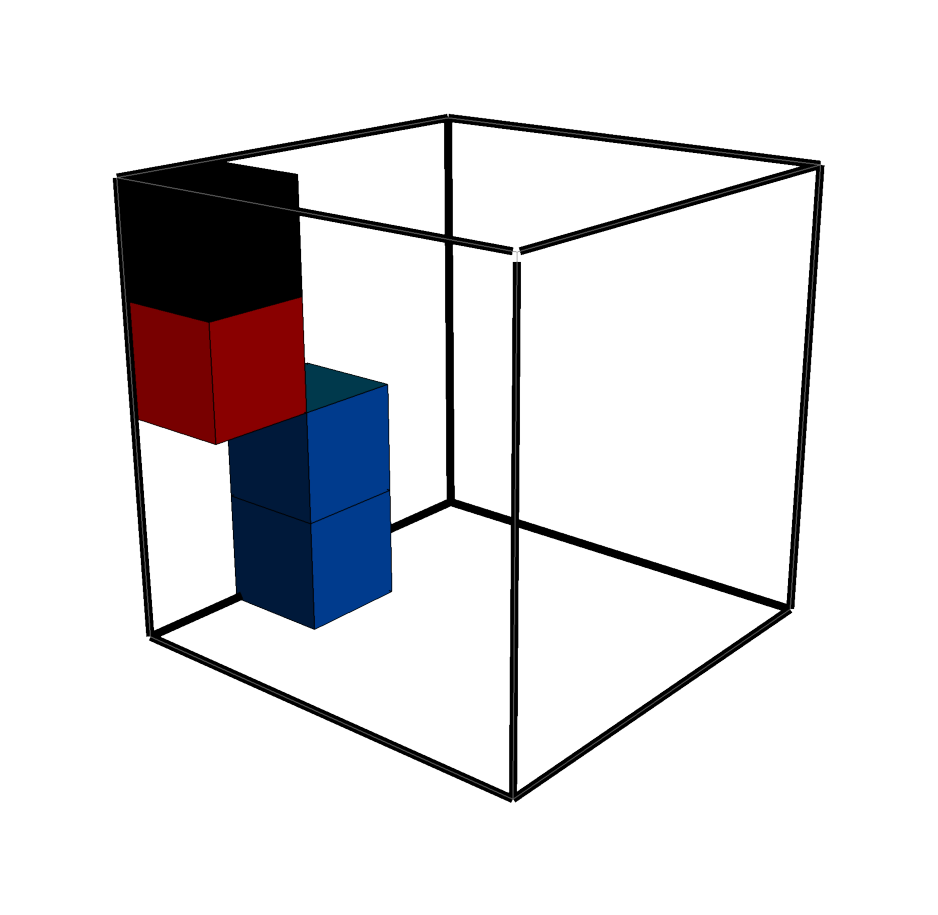
\includegraphics[height=3cm]{img/3q-4c-si-3}
	\hfill
	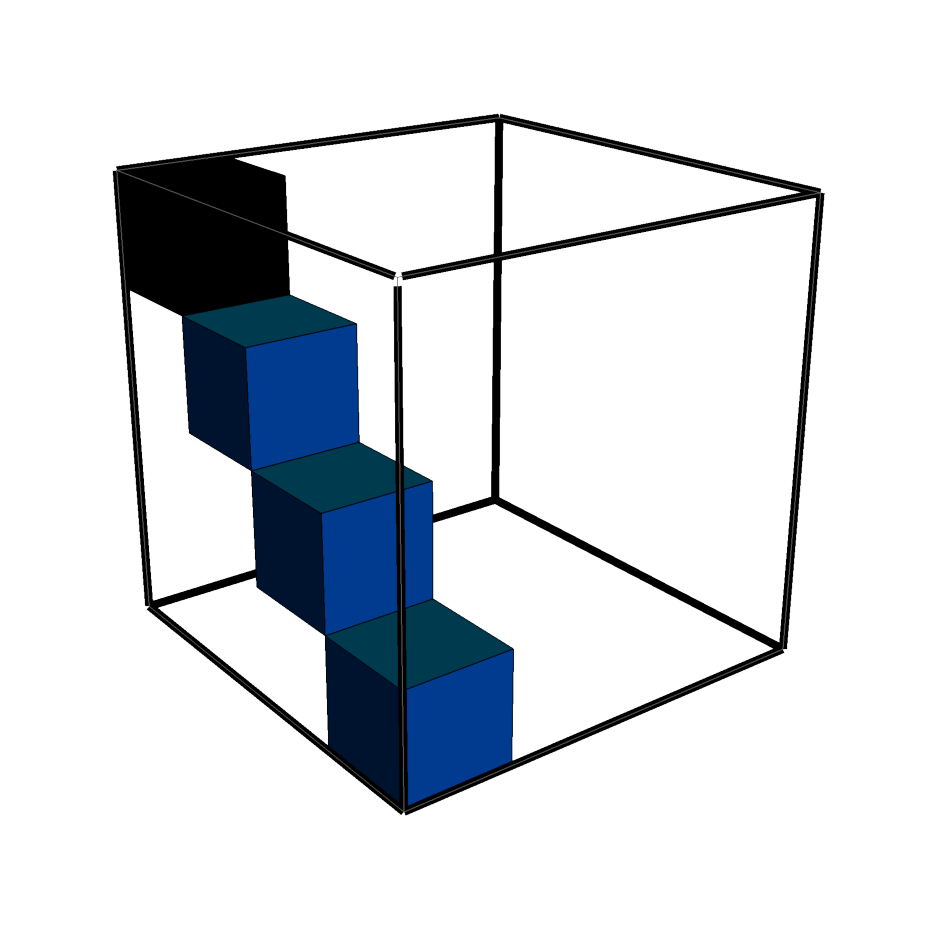
\includegraphics[height=3cm]{img/3q-4c-si-4}
	\hfill
	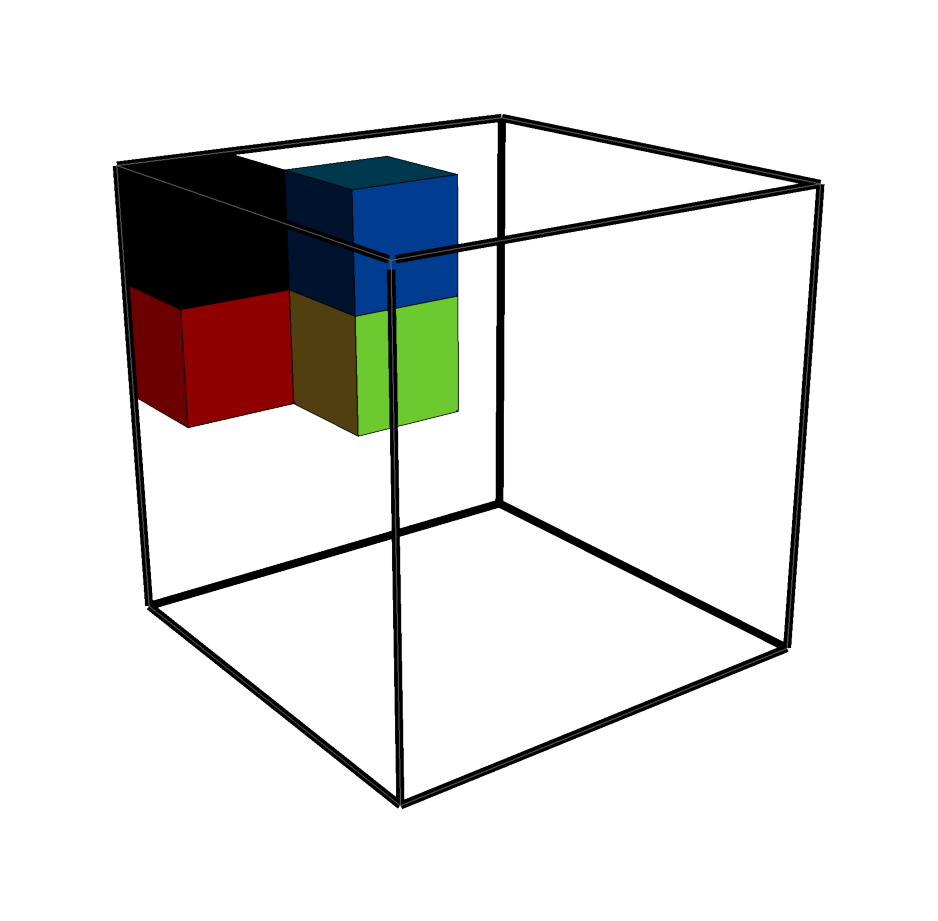
\includegraphics[height=3cm]{img/3q-4c-si-5}
	\hfill
	\vfill
	\hfill
	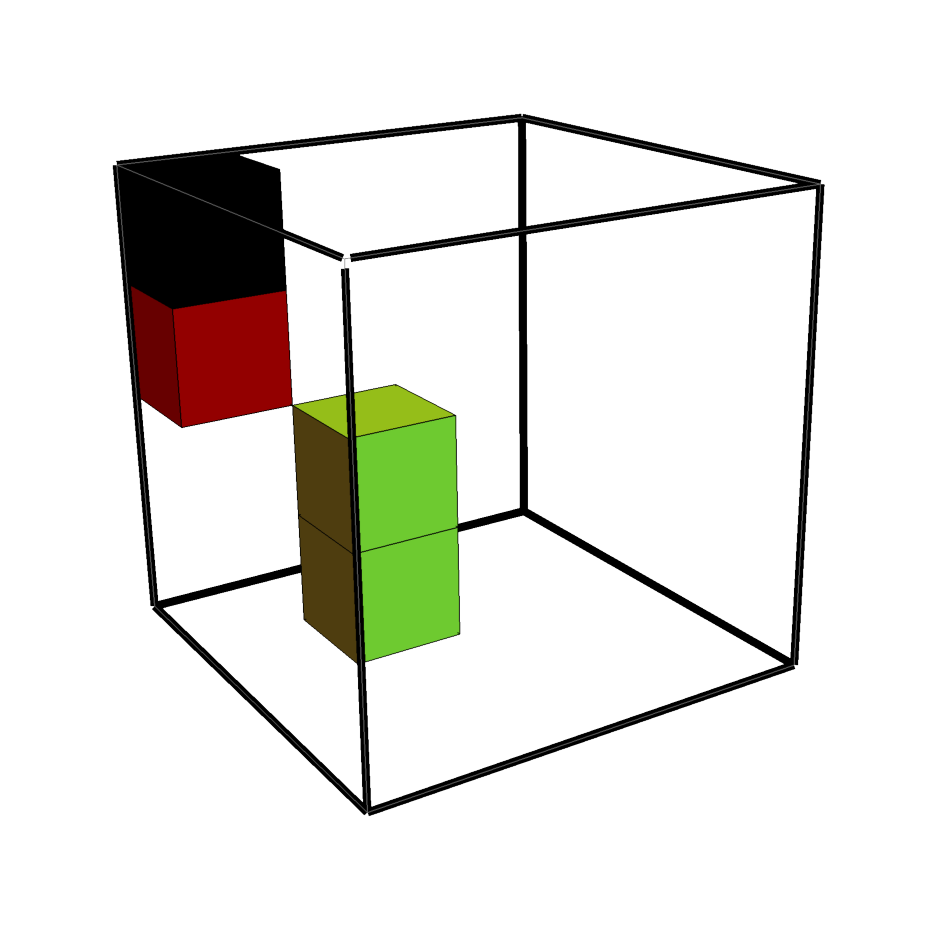
\includegraphics[height=3cm]{img/3q-4c-no-1}
	\hfill
	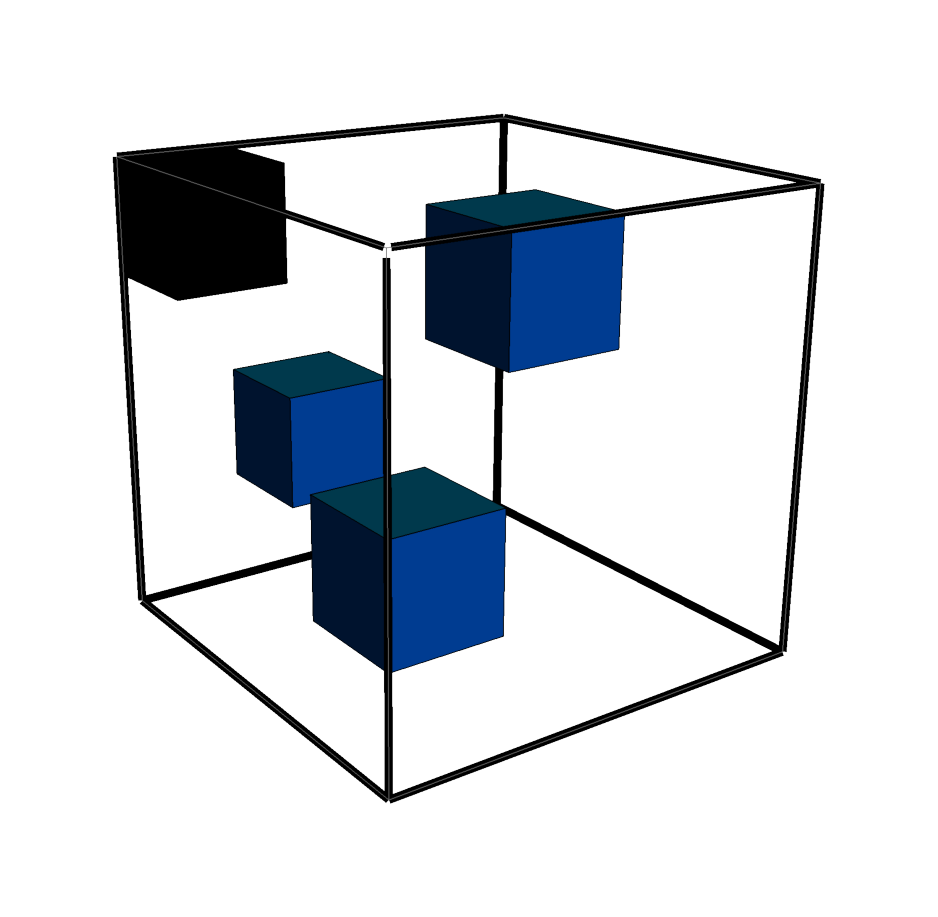
\includegraphics[height=3cm]{img/3q-4c-no-2}
	\hfill
	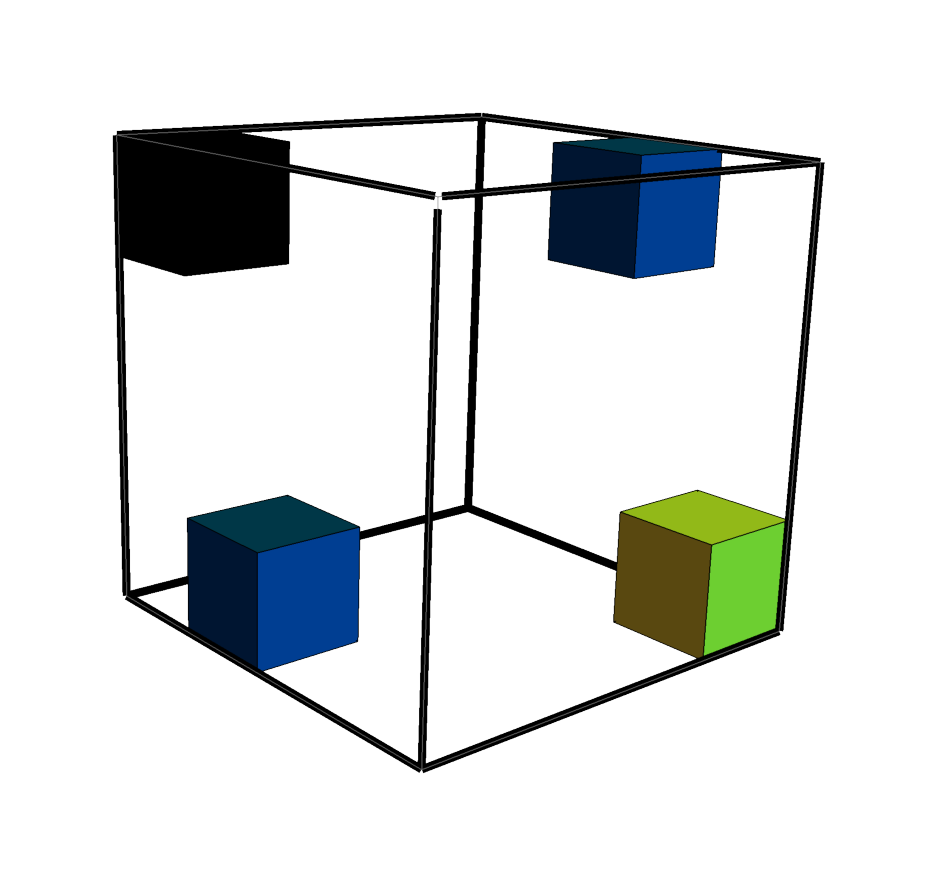
\includegraphics[height=3cm]{img/3q-4c-no-3}
	\hfill
	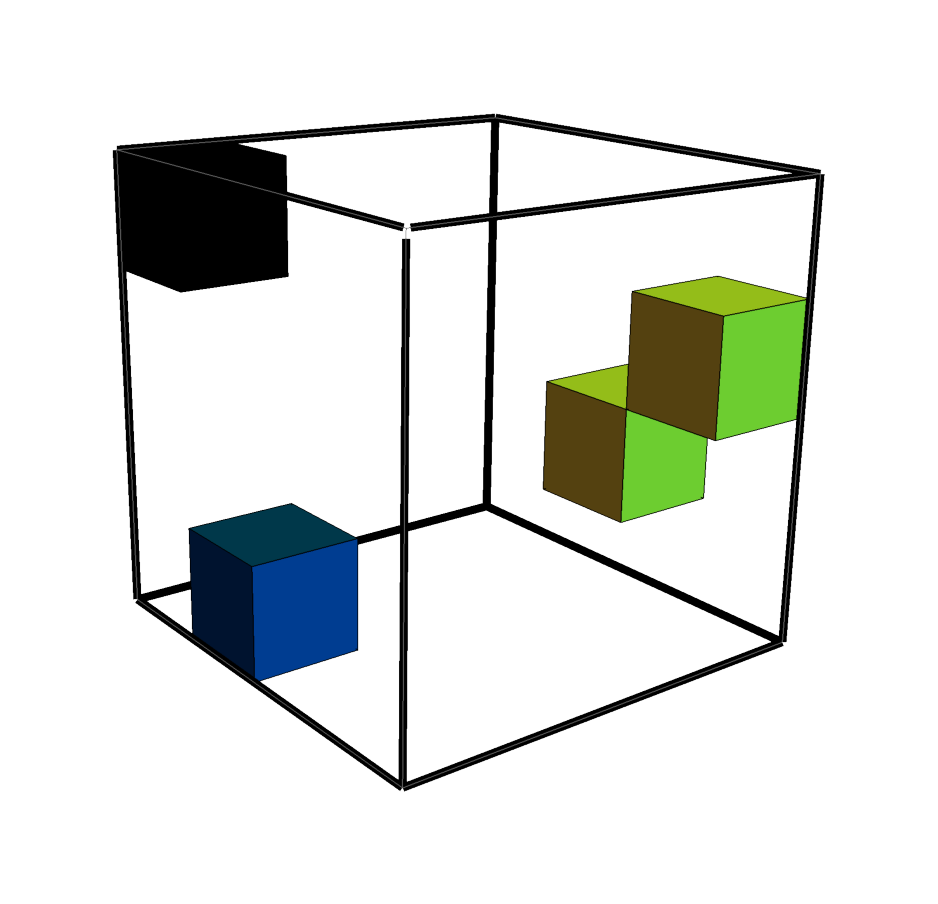
\includegraphics[height=3cm]{img/3q-4c-no-4}
	\hfill
	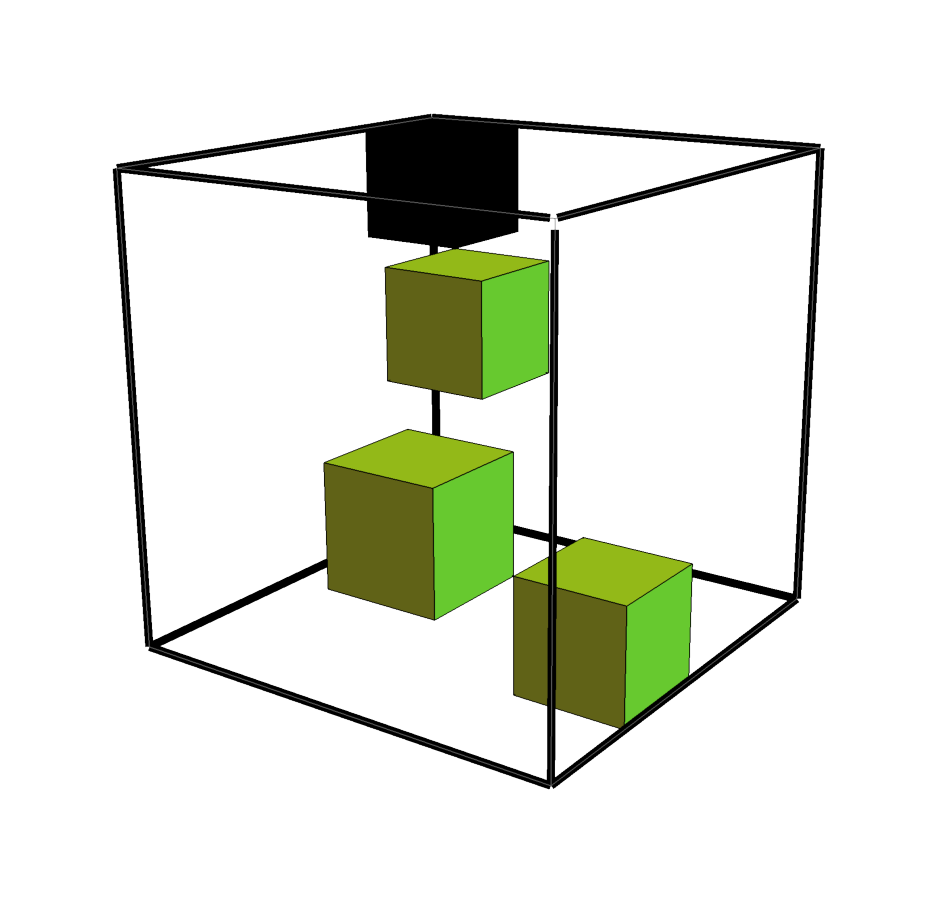
\includegraphics[height=3cm]{img/3q-4c-no-5}
	\hfill \hfill
	\caption{One element of every of the 10 equivalence
	classes of the 3-qubits 2-invariant-components quantum channels.}
	\label{fig:QC-3q-4c}
\end{figure}
% }}}

In principle, the rainbow hypothesis makes a connection between the 
channels presented and channels that leave invariant 16, 32 and 64
components. Therefore, we're currently inferring those quantum channels
from those presented in figures \ref{fig:QC-3q-1c}, \ref{fig:QC-3q-2c} and
\ref{fig:QC-3q-4c}. It is only necessary to find one element in an 
equivalence class because the rest are found by particle swaps 
and permutation of individual components.
% }}}
\cpnote{Sería importante discutir como se comportan todas las hipotesis que hiciste 
para dos qubits en el caso de 3 qubits}
% }}}

\section*{Are this channels a subset of Pauli diagonal channels constant on axes?} % {{{


We explored if the quantum channels of our study have a containance relation
with the subset of Pauli diagonal
channels constant on axes \cite{nathanson2007pauli}, let us call them
$\mathcal{R}$.  We concluded that only Kraus rank $4$ channels of the ones
under study are candidates to
be in $\mathcal{R}$, in fact we are convinced that all of them are in, but are
still working in the proof \cpnote{David is convinced, the rest of us
have no idea}. To see this
let us analyse the action of Ruskai's maps on arbitrary density matrices
\begin{align}
	\rho \mapsto \frac{1}{d}\qty[\1 + \sum _{J=1}^{d+1} \sum _{j=1}^{d-1}
	\lambda_J v_{Jj}W_J^j],
	\label{eq:ruskai-rho}
\end{align}
where $\Lambda_J$ are the eigenvalues of a given Ruskai map. \fxnote{Por fas
corrige la argumentacion a partir de la modificacion a la ecuacion} where $d$
is the dimension of the Hilbert space of the system and $W_J^j$ \fxnote{JA, ojo
que los $W_J$ generan un grupo ciclico, mas no generadores de MUBs, uno
construye los $W_J$ usando MUBs!. Por fas mejor mete la definicion de $W_J$.}
are generators of a mutually unbiased bases (MUB) for $\mathbb{C}^{d}$.  Then,
the action of a Pauli diagonal channel constant on axes on a $\rho$ of the form
\eqref{eq:ruskai-rho} is to take $v_{Jj}\mapsto (s+t_J)v_{Jj}$. The eigenvalues
of a Pauli diagonal channel are 1 and $\lambda _J=s+t_J$. Note that there are
$d+1$ eigenvalues $\lambda_J$, and every eigenvalue has degeneration $d-1$. 

In order to construct a channel of ours from a 
Pauli diagonal channel $\lambda_J$ must be equal to one or zero. Our
quantum channels have a power-of-2 rank. On the other hand, 
the rank of a Pauli diagonal channel is $1+3k$ ($k\in \mathbb{Z}^+$,
$1\leq k\leq d+1$),
therefore there are subsets of our quantum channels that cannot be  
Pauli diagonal channels constant on axes. For example, a quantum channel of 2 qubits 
($d=4$) that leaves invariant 8 components in $\rho$ has rank 8, and
there's not a $k$ for which the rank of a Pauli diagonal channel may be 8.


%\cpnote{Creo que eso ya lo teníamos claro. Sería bueno que discutieramos pues 
%me gustaría dar mas seguridades. De hecho tu argumento me parece una prueba, pero quizá
%lo tengamos que refinar. Planeemos una reunion pronto con el resto del combo para ver esto.
%Obvio, creo, si hay intersección, pero no son los mismos.}
% }}}
\section*{To-do} % {{{
In order to fully understand our results and generalize this kind of maps 
for $n$ qubits we propose the following:
\begin{enumerate}
\item Investigate the Kraus operator representation of this quantum channels.
\item Investigate the Schmidt spectrum of the Choi matrix.
\item Investigate the Jamiolkowski isomorphism to find an equivalence between
CP and the empirical rules listed previously.
\item Use our current results to propose an efficient way to do numerical
analysis to find 3-qubit quantum channels that leave 8 components invariant.
\end{enumerate}
% }}}
\bibliographystyle{unsrt}
\bibliography{references}
\vfill

\end{document}
